\documentclass[tikz,border=5pt]{standalone}

% =========================================================
% 基础数学与量子记号
% =========================================================
\usepackage{amsmath}        % 数学公式
\usepackage{braket}         % \ket{}, \bra{}
\usepackage{newtxtext,newtxmath} % Times-like 正文 + 数学字体（PRA/PRL 风格）

% =========================================================
% TikZ 库
% =========================================================
\usetikzlibrary{
  arrows.meta,              % 现代箭头（Stealth 等）
  decorations.pathmorphing  % 备用：波浪线等（目前未用）
}

% =========================================================
% 全局数学公式样式
% 所有 $...$ 默认使用 displaystyle
% 让 \Omega, \Delta, V_{ij} 更饱满
% =========================================================
\everymath{\displaystyle}

\begin{document}

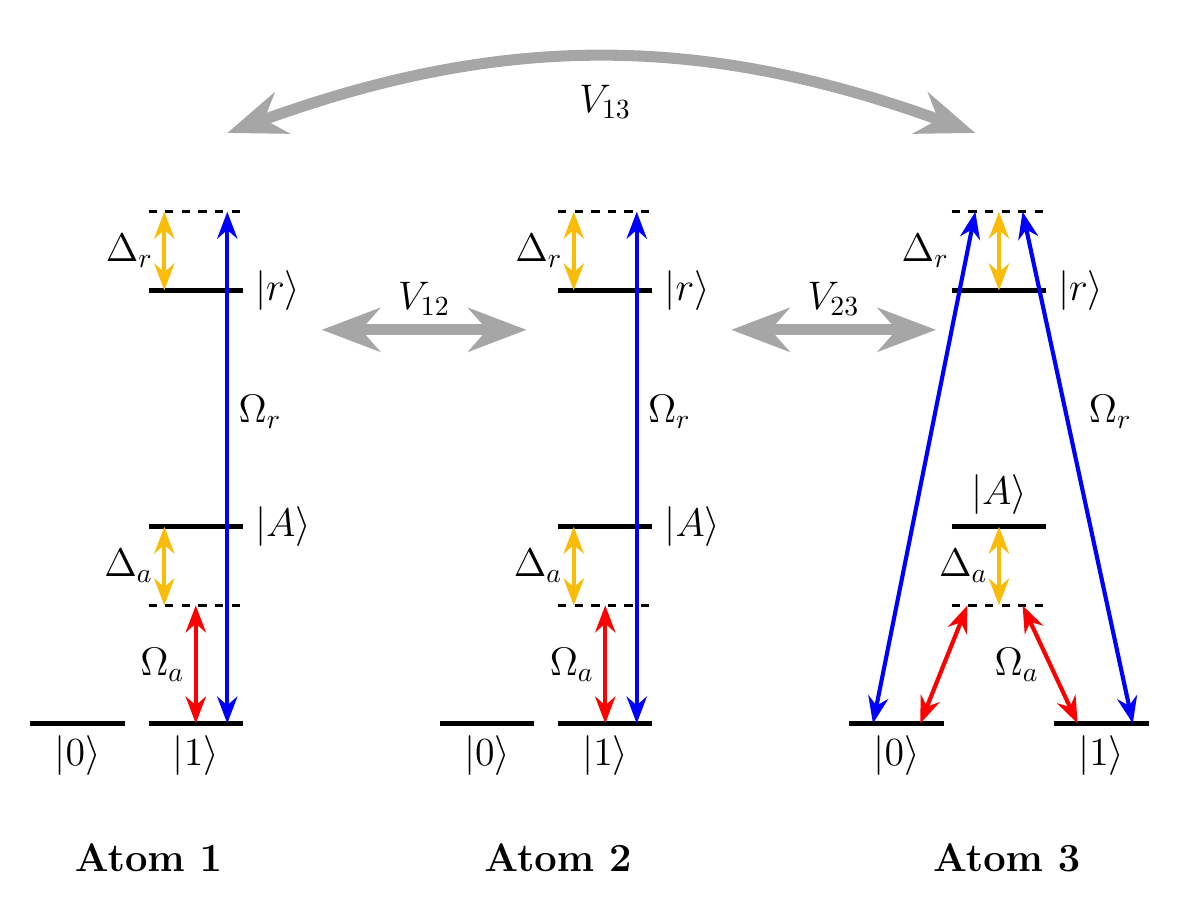
\begin{tikzpicture}[
    % =====================================================
    % 样式定义（只管“画笔属性”，不管几何）
    % =====================================================
    level/.style={
        line width=2pt            % 实能级：较粗实线
    },
    vlevel/.style={
        line width=1.2pt,
        dashed                   % 虚能级：细虚线
    },
    laser/.style={
        <->,
        line width=1.5pt,
        >=Stealth                % 激光：双向箭头
    },
    detune/.style={
        <->,
        line width=1.5pt,
        >=Stealth                % 失谐 Δ：双向箭头
    },
    int/.style={
        <->,
        line width=4pt,
        draw=gray!70,
        >=Stealth                % Rydberg 相互作用
    },
    % =====================================================
    % 所有 node 的统一字体设置
    % =====================================================
    every node/.style={
        font=\Large\bfseries,
        text=black
    }
]

% =========================================================
% 全局几何参数（控制整体布局）
% =========================================================

% -------- 三个原子的横向位置 --------
\def\xA{0}        % Atom 1
\def\xB{5.2}      % Atom 2
\def\xC{10.4}     % Atom 3

% -------- 能级高度 --------
\def\yzero{0}     % |0>, |1> 基态
\def\yA{2.5}      % |A> 实能级
\def\yr{5.5}      % |r> 实能级

% -------- 虚能级高度 --------
\def\yAv{1.5}     % |A> 对应虚能级
\def\yrv{6.5}     % |r> 对应虚能级

% =========================================================
% ===================== Atom 1 =============================
% =========================================================

% -------- 基态 |0>, |1> --------
\draw[level] (\xA,\yzero) -- ++(1.2,0)
    node[midway,below] {$\ket{0}$};

\draw[level] (\xA+1.5,\yzero) -- ++(1.2,0)
    node[midway,below] {$\ket{1}$};

% -------- 激发态 |A>, |r> --------
\draw[level] (\xA+1.5,\yA) -- ++(1.2,0)
    node[right] {$\ket{A}$};

\draw[level] (\xA+1.5,\yr) -- ++(1.2,0)
    node[right] {$\ket{r}$};

% -------- 虚能级（激光失谐后的能级） --------
\draw[vlevel] (\xA+1.5,\yAv) -- ++(1.2,0);
\draw[vlevel] (\xA+1.5,\yrv) -- ++(1.2,0);

% -------- 激光驱动 --------
\draw[laser, red]
    (\xA+2.1,\yzero) -- (\xA+2.1,\yAv)
    node[midway,left] {$\Omega_a$};

\draw[laser, blue]
    (\xA+2.5,\yzero) -- (\xA+2.5,\yrv)
    node[midway,right,yshift=20px] {$\Omega_r$};

% -------- 失谐标注 Δ --------
\draw[detune,yellow!50!orange]
    (\xA+1.7,\yA) -- (\xA+1.7,\yAv)
    node[midway,left] {$\Delta_a$};

\draw[detune,yellow!50!orange]
    (\xA+1.7,\yr) -- (\xA+1.7,\yrv)
    node[midway,left] {$\Delta_r$};

% -------- 原子标签 --------
\node at (\xA+1.5,-1.7) {Atom 1};

% =========================================================
% ===================== Atom 2 =============================
% =========================================================
% （结构与 Atom 1 完全一致，仅横向平移）

\draw[level] (\xB,\yzero) -- ++(1.2,0)
    node[midway,below] {$\ket{0}$};

\draw[level] (\xB+1.5,\yzero) -- ++(1.2,0)
    node[midway,below] {$\ket{1}$};

\draw[level] (\xB+1.5,\yA) -- ++(1.2,0)
    node[right] {$\ket{A}$};

\draw[level] (\xB+1.5,\yr) -- ++(1.2,0)
    node[right] {$\ket{r}$};

\draw[vlevel] (\xB+1.5,\yAv) -- ++(1.2,0);
\draw[vlevel] (\xB+1.5,\yrv) -- ++(1.2,0);

\draw[laser, red]
    (\xB+2.1,\yzero) -- (\xB+2.1,\yAv)
    node[midway,left] {$\Omega_a$};

\draw[laser, blue]
    (\xB+2.5,\yzero) -- (\xB+2.5,\yrv)
    node[midway,right,yshift=20px] {$\Omega_r$};

\draw[detune,yellow!50!orange]
    (\xB+1.7,\yA) -- (\xB+1.7,\yAv)
    node[midway,left] {$\Delta_a$};

\draw[detune,yellow!50!orange]
    (\xB+1.7,\yr) -- (\xB+1.7,\yrv)
    node[midway,left] {$\Delta_r$};

\node at (\xB+1.5,-1.7) {Atom 2};

% =========================================================
% ===================== Atom 3 (Λ 型) ======================
% =========================================================

% -------- 基态 |0>, |1> --------
\draw[level] (\xC,\yzero) -- ++(1.2,0)
    node[midway,below] {$\ket{0}$};

\draw[level] (\xC+2.6,\yzero) -- ++(1.2,0)
    node[midway,below] {$\ket{1}$};

% -------- 激发态 --------
\draw[level] (\xC+1.3,\yA) -- ++(1.2,0)
    node[midway,above] {$\ket{A}$};

\draw[level] (\xC+1.3,\yr) -- ++(1.2,0)
    node[right] {$\ket{r}$};

% -------- 虚能级 --------
\draw[vlevel] (\xC+1.3,\yAv) -- ++(1.2,0);
\draw[vlevel] (\xC+1.3,\yrv) -- ++(1.2,0);

% -------- Λ 型激光 --------
\draw[laser, blue]
    (\xC+0.3,\yzero) -- (\xC+1.6,\yrv);

\draw[laser, blue]
    (\xC+3.6,\yzero) -- (\xC+2.2,\yrv)
    node[midway,right,yshift=20px] {$\Omega_r$};

\draw[laser, red]
    (\xC+1.5,\yAv) -- (\xC+0.9,\yzero);

\draw[laser, red]
    (\xC+2.2,\yAv) -- (\xC+2.9,\yzero)
    node[midway,left] {$\Omega_a$};

% -------- 失谐 --------
\draw[detune,yellow!50!orange]
    (\xC+1.9,\yA) -- (\xC+1.9,\yAv)
    node[midway,left] {$\Delta_a$};

\draw[detune,yellow!50!orange]
    (\xC+1.9,\yr) -- (\xC+1.9,\yrv)
    node[midway,left,xshift=-14pt] {$\Delta_r$};

\node at (\xC+2,-1.7) {Atom 3};

% =========================================================
% ================= Rydberg 相互作用 =======================
% =========================================================

% -------- 最近邻相互作用 --------
\draw[int]
    (\xA+3.7,\yrv-1.5) -- (\xB+1.1,\yrv-1.5)
    node[midway,above] {$V_{12}$};

\draw[int]
    (\xB+3.7,\yrv-1.5) -- (\xC+1.1,\yrv-1.5)
    node[midway,above] {$V_{23}$};

% -------- 远程相互作用（弯曲箭头） --------
\draw[int]
    (\xA+2.5,\yrv+1)
    to[out=20, in=160]
    (\xC+1.6,\yrv+1)
    node at (\xB+2.1,\yrv+1.4) {$V_{13}$};

\end{tikzpicture}

\end{document}
